\newpage
\appendix
\section{C\# REST-API Implementierung}
\begin{lstlisting}[language={[Sharp]C}, caption={REST-API C\# Implementierung}, captionpos=b, label={fig:restApi}]
    #region method
    /// <summary>
    /// The URL field is used to load the current data from the website into a JSON format via the RestAPI. 
    /// The <see cref="HttpClient"/> converts this into the corresponding class structure and returns it as <see cref="List{Root}"/>.
    /// </summary>
    /// <returns><see cref="List{Root}"/></returns>
    public List<Root> GetResult()
    {
        var t = Task.Run(() => GetResultAsync(Url));
        t.Wait();
        return t.Result;
    }

    [HttpGet, Route("Results")]
    public async Task<List<Root>> GetResultAsync(string url)
    {
        // Call asynchronous network methods in a try/catch block to handle exceptions.
        try
        {
            return await httpClient.GetFromJsonAsync<List<Root>>(url);
        }
        catch (HttpRequestException e)
        {
            Programm.LogService.LogError(e);
        }
        return null;
    }
    #endregion
\end{lstlisting}
\section{JSON Beispiel}
\begin{figure}[H]
    \centering
    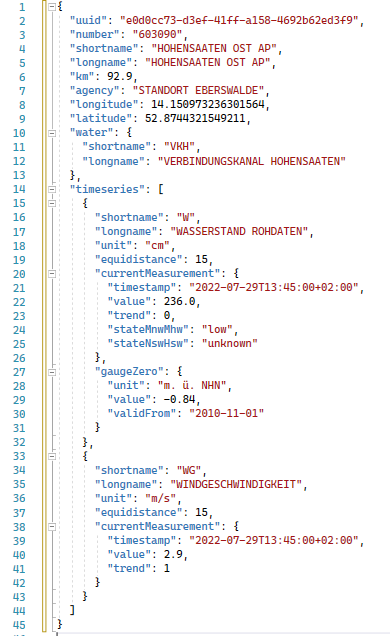
\includegraphics[width=0.7\linewidth]{figures/Json_example.PNG} 
    \caption{JSON Beispiel}
    \label{fig:jsonExample}
\end{figure}
\newpage
\section{Klassendiagramm}
\begin{figure}[H]
    \centering
    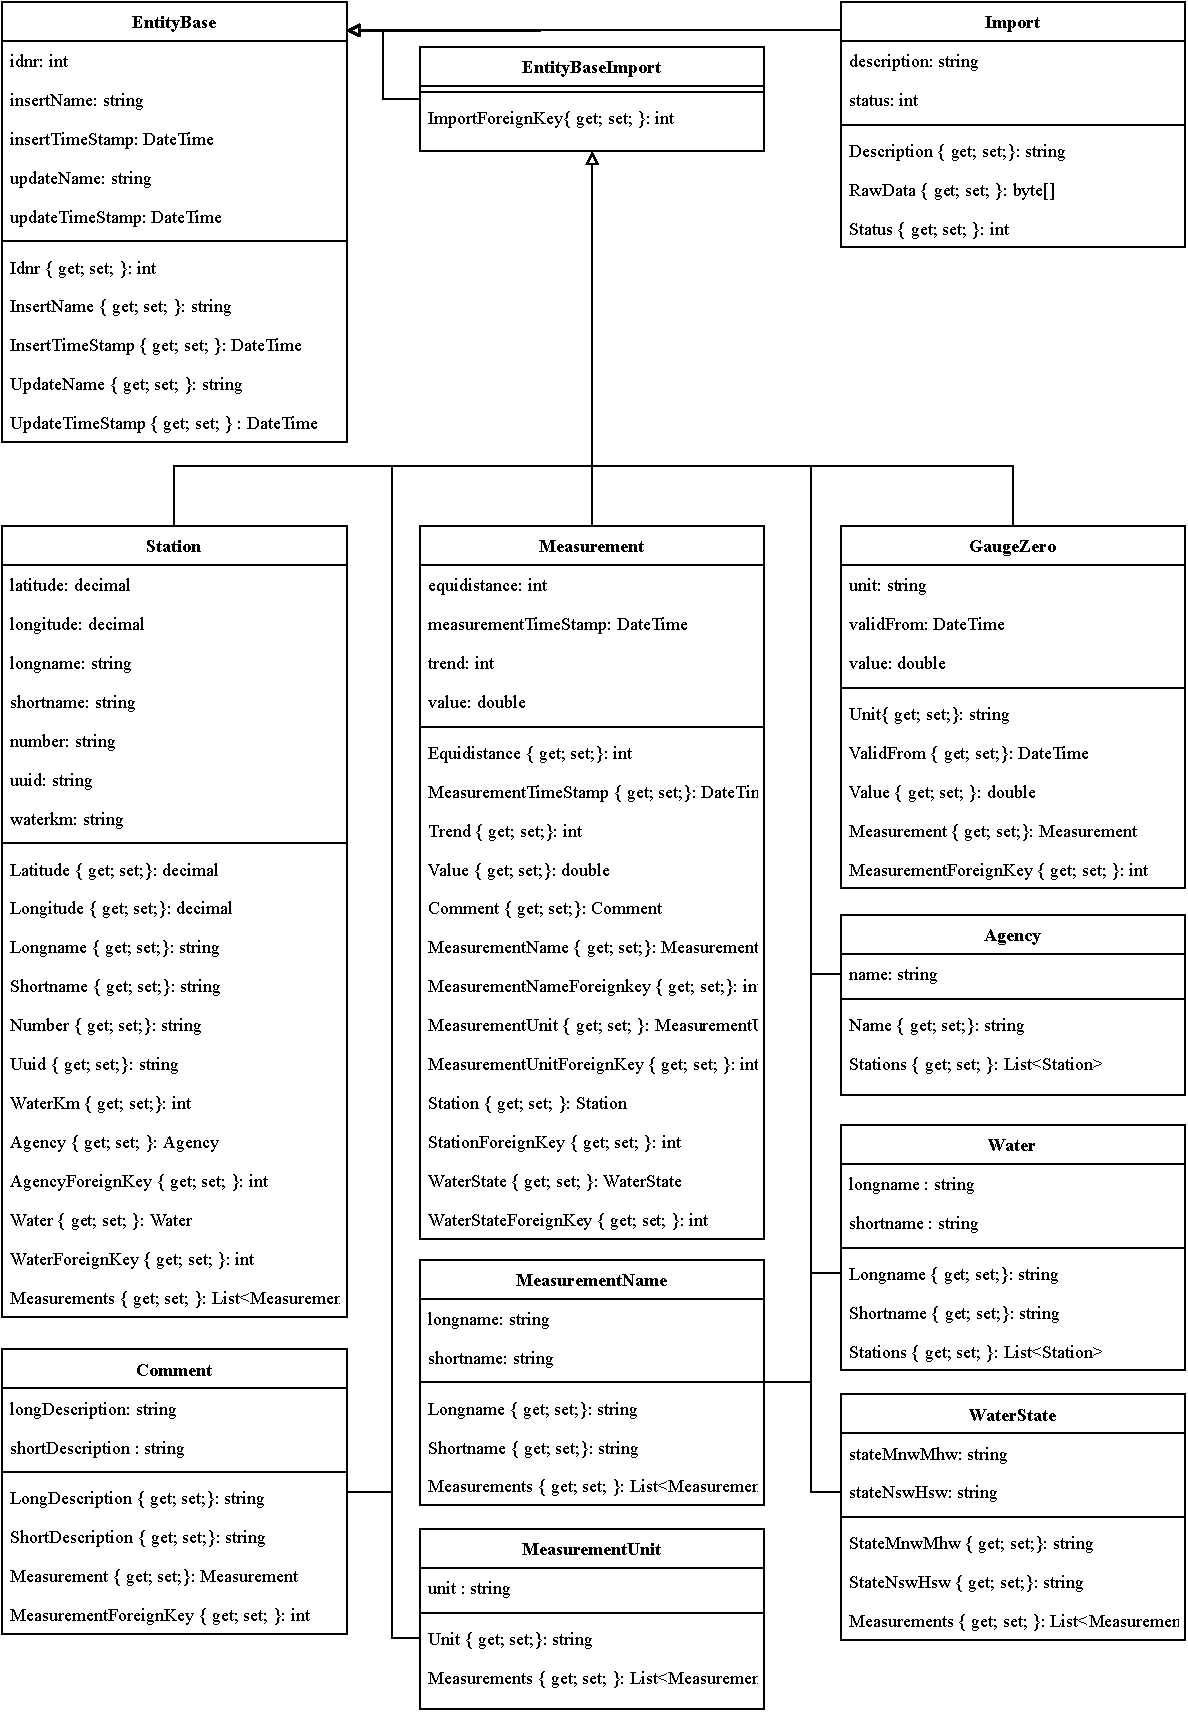
\includegraphics[width=0.85\linewidth]{figures/classDiagram.pdf}
    \caption[Klassendiagramm]{Klassendiagramm}   
    \label{fig:classDiagramm}
\end{figure}

\section{Selbstständigkeitserklärung Jan Lippemeier}
Ich erkläre, dass
\begin{itemize}
    \item[o] alle sinngemäßen Übernahmen aus Arbeiten Dritter mit der Quellenangabe gekennzeichnet sind,
    \item[o] alle wörtlichen Übernahmen von Textpassagen aus Arbeiten Dritter durch Anführungszeichen und ausführliche Angabe der Belegstelle als Zitat gekennzeichnet sind,
    \item[o] die vorliegende Arbeit selbständig unter Verwendung der im experimentellen Teil genannten Methoden angefertigt wurde und
    \item[o] Primärdaten von Experimenten der Arbeit unverändert und in geeigneter Form beigefügt sind.
\end{itemize}
\vspace*{0.5cm}
\begin{flushleft}
  \begin{table}[H]
      \begin{tabular}{l  l }
          \hline 
          Ort und Datum \hspace*{3cm}  & Unterschrift \hspace*{5cm}
      \end{tabular}    
  \end{table}
\end{flushleft}

\newpage

\section{Selbstständigkeitserklärung Henrik Lohre}
Ich erkläre, dass
\begin{itemize}
    \item[o] alle sinngemäßen Übernahmen aus Arbeiten Dritter mit der Quellenangabe gekennzeichnet sind,
    \item[o] alle wörtlichen Übernahmen von Textpassagen aus Arbeiten Dritter durch Anführungszeichen und ausführliche Angabe der Belegstelle als Zitat gekennzeichnet sind,
    \item[o] die vorliegende Arbeit selbständig unter Verwendung der im experimentellen Teil genannten Methoden angefertigt wurde und
    \item[o] Primärdaten von Experimenten der Arbeit unverändert und in geeigneter Form beigefügt sind.
\end{itemize}
\vspace*{0.5cm}
\begin{flushleft}
  \begin{table}[H]
      \begin{tabular}{l  l }
          \hline 
          Ort und Datum \hspace*{3cm}  & Unterschrift \hspace*{5cm}
      \end{tabular}    
  \end{table}
\end{flushleft}

\newpage
\section{Selbstständigkeitserklärung Dennis Reinhardt}
Ich erkläre, dass
\begin{itemize}
    \item[o] alle sinngemäßen Übernahmen aus Arbeiten Dritter mit der Quellenangabe gekennzeichnet sind,
    \item[o] alle wörtlichen Übernahmen von Textpassagen aus Arbeiten Dritter durch Anführungszeichen und ausführliche Angabe der Belegstelle als Zitat gekennzeichnet sind,
    \item[o] die vorliegende Arbeit selbständig unter Verwendung der im experimentellen Teil genannten Methoden angefertigt wurde und
    \item[o] Primärdaten von Experimenten der Arbeit unverändert und in geeigneter Form beigefügt sind.
\end{itemize}
\vspace*{0.5cm}
\begin{flushleft}
  \begin{table}[H]
      \begin{tabular}{l  l }
          \hline 
          Ort und Datum \hspace*{3cm}  & Unterschrift \hspace*{5cm}
      \end{tabular}    
  \end{table}
\end{flushleft}


\newpage